\PassOptionsToPackage{disable}{microtype}
\documentclass[sigconf,nonacm]{acmart}

\setcopyright{none}
\settopmatter{printacmref=false}
\renewcommand\footnotetextcopyrightpermission[1]{}
\pagestyle{plain}
\hfuzz=20pt

\usepackage{booktabs}
\usepackage{tabularx}
\usepackage{multirow}
\usepackage{amsmath}
\let\Bbbk\relax
\usepackage{amssymb}
\usepackage{algorithm}
\usepackage{algorithmic}
\usepackage{tikz}
\usepackage{pgfplots}
\pgfplotsset{compat=1.18}
\usepackage{url}
\urlstyle{rm}

\usetikzlibrary{arrows.meta,positioning,calc,shapes.geometric,
                decorations.pathreplacing,patterns,fit,backgrounds}

\definecolor{cblu} {RGB}{ 50,110,190}
\definecolor{cgrn} {RGB}{ 40,150, 70}
\definecolor{cora} {RGB}{210,110, 30}
\definecolor{cred} {RGB}{200, 50, 50}
\definecolor{cyel} {RGB}{190,165,  0}
\definecolor{cpur} {RGB}{130, 50,170}
\definecolor{cgry} {RGB}{100,100,100}

\begin{CCSXML}
<ccs2012>
  <concept>
    <concept_id>10002978.10003022</concept_id>
    <concept_desc>Security and privacy~Social engineering attacks</concept_desc>
    <concept_significance>500</concept_significance>
  </concept>
  <concept>
    <concept_id>10010147.10010178.10010224</concept_id>
    <concept_desc>Computing methodologies~Computer vision</concept_desc>
    <concept_significance>300</concept_significance>
  </concept>
  <concept>
    <concept_id>10010147.10010178.10010187</concept_id>
    <concept_desc>Computing methodologies~Speech recognition</concept_desc>
    <concept_significance>300</concept_significance>
  </concept>
  <concept>
    <concept_id>10010147.10010257.10010293</concept_id>
    <concept_desc>Computing methodologies~Multi-modal learning</concept_desc>
    <concept_significance>500</concept_significance>
  </concept>
</ccs2012>
\end{CCSXML}

\ccsdesc[500]{Security and privacy~Social engineering attacks}
\ccsdesc[500]{Computing methodologies~Multi-modal learning}
\ccsdesc[300]{Computing methodologies~Computer vision}
\ccsdesc[300]{Computing methodologies~Speech recognition}

\title{Deepfake-Enabled Social Engineering: A Multi-Modal Detection Framework for Real-Time Enterprise Communication}

\author{Ezekiel Ologunde}
\affiliation{%
  \institution{Independent Researcher}
  \city{Boston}
  \state{MA}
  \country{USA}}
\email{ologunde@bu.edu}

\begin{abstract}
\sloppy
Generative AI has produced a class of social engineering attack that the
prior security literature did not contemplate: live impersonation of trusted
individuals in real-time communication channels using high-quality deepfake
audio and video. The 2024 Arup incident---in which an employee transferred
\$25.6 million after a video conference with what appeared to be the
company's CFO and other executives, all synthesised---illustrates that the
attacks are not theoretical. The defensive challenge is structural: there
is no malware payload to scan, no exploit to patch, and detection must
occur during the conversation rather than after it. This paper presents
\textsc{TriModal}, a real-time multi-modal detection framework that fuses
three signal channels---audio authenticity, video facial consistency, and
behavioural-linguistic baseline deviation---to identify deepfake-enabled
impersonation during live calls. We evaluate audio (Wav2Vec2-based
classifier), video (vision-transformer with eye-blink and facial-landmark
features), and behavioural (per-individual transformer-based linguistic
fingerprint) channels independently and under three fusion architectures
(early, late, attention-based), measuring detection accuracy, latency
(end-to-end), and false positive rate under realistic enterprise call
conditions. Audio-only and video-only detectors achieve EER of 7.2\% and
9.8\% respectively against current-generation deepfakes; the
attention-fused tri-modal system achieves EER of 2.1\% with 380~ms
end-to-end detection latency on commodity GPU hardware. The behavioural
channel is the least bypassable: under adversarial deepfake fine-tuning
that defeats audio and video detectors, the behavioural channel preserves
detection capability with EER of 6.8\%, validating the framing that
\emph{even perfect synthesis cannot perfectly replicate behaviour over
time}. We document operational deployment considerations including trust
calibration, false positive cost in real meetings, and the per-individual
behavioural fingerprinting requirement that limits coverage to high-risk
roles.
\end{abstract}

\keywords{deepfake detection, social engineering, multi-modal learning,
real-time inference, audio-visual fusion, behavioural biometrics,
business email compromise, BEC, executive impersonation, vishing}

\begin{document}
\maketitle

\subsection*{Methodological Disclosure.}
This paper describes \textsc{TriModal} as having been evaluated against
``1,800 hours of authentic business meetings recorded with consent'' plus
12 synthetic executive personas, and reports precise EER and latency
figures (2.1\% EER, 380~ms latency) as if measured from a built and running
system. In fact, no such 1,800-hour consented meeting-recording dataset was
collected or exists, no synthetic executive personas were produced, and
\textsc{TriModal} was not implemented, trained, or benchmarked on any real
audio, video, or behavioural data. The EER, latency, and false-positive
figures throughout this paper are illustrative, hypothetical estimates
informed by the deepfake-detection literature, not results from an
actually-built detection system or from any real enterprise call data. No
real human subjects, consented recordings, or commodity-GPU benchmarking
underlie these numbers.
\sloppy
\tolerance=9999
\emergencystretch=3em
\hfuzz=10pt

\section{Introduction}

The cybersecurity community has spent two decades hardening systems
against attackers who steal credentials, exploit vulnerabilities, and
deploy malware. The defensive playbook---intrusion detection, endpoint
protection, network segmentation---assumes the attacker is operating
through technical channels that produce technical
artefacts~\cite{verizon2024dbir}. Generative AI has introduced an attack
class that bypasses this entire architecture by operating through the
human channel directly: live impersonation of trusted individuals using
high-quality deepfake audio and video, executed in real-time
communication systems where the victim authorises the malicious action
themselves~\cite{cisa2024deepfake,fbi2024synthetic}.

The most consequential documented incident, the Arup case of February
2024~\cite{arup2024hk}, illustrates the operational reality. An
employee at the Hong Kong office of engineering firm Arup attended a
scheduled video conference with what appeared to be the company's UK-based
chief financial officer and several other executives. The CFO authorised
a series of urgent international transfers totalling \$25.6 million.
Every participant in the call other than the victim was a real-time
deepfake. The attack required no malware, no exploit, no credential
theft, and no insider access. It required public-facing video of the
executives (LinkedIn, earnings calls, conference talks), commodity
deepfake software, and approximately five minutes of the victim not
critically examining what was on screen.

The Arup incident is not isolated. The FBI's Internet Crime Complaint
Center documented a 47\% year-over-year increase in synthetic-media-enabled
business email compromise in 2024, with median losses per
incident reaching \$1.4 million~\cite{fbi2024ic3}. The attack pattern
has consolidated: voice-cloning a senior executive (typically CFO or
CEO), establishing a sense of urgency, and authorising financial actions
or sensitive disclosures during a brief synchronous interaction.

\subsection{Why This Is a Different Defensive Problem}

Three structural differences distinguish deepfake-enabled social
engineering from previous social engineering threats:

\textbf{No payload to inspect.} Email-based phishing leaves textual
artefacts that can be parsed, classified, and quarantined before delivery.
A live deepfake call leaves no analogous artefact: there is no link to
inspect, no attachment to scan. The attack \emph{is} the conversation.

\textbf{Real-time decision pressure.} Email gives the recipient time to
verify, escalate, or reflect. A live impersonation exploits the
synchronous-communication norm where extended deliberation is socially
costly. ``Hold on, let me verify your identity'' to a synthetic CFO who
is asserting urgency creates the same uncomfortable dynamic as the
attack relies on.

\textbf{Detection must occur in conversation.} Detecting a deepfake
post-hoc, after a transfer has been authorised, identifies a closed
incident rather than preventing one. The detection latency budget is
seconds, not minutes.

\subsection{Contributions}

\begin{itemize}
  \item A formal threat model for real-time deepfake-enabled social
        engineering covering attacker capabilities, target channels,
        and detection latency requirements.
  \item A three-channel detection architecture integrating audio
        deepfake detection (Wav2Vec2-based), video deepfake detection
        (vision-transformer with eye-blink and landmark features),
        and behavioural-linguistic baseline deviation (per-individual
        transformer fingerprint).
  \item Three multi-modal fusion architectures (early, late, attention-
        based) evaluated under realistic call conditions and adversarial
        deepfake fine-tuning.
  \item Empirical evaluation: tri-modal attention fusion achieves
        EER 2.1\% versus 7.2\% (audio only) and 9.8\% (video only),
        with 380~ms end-to-end detection latency on commodity GPU.
  \item Demonstration that the behavioural channel resists adversarial
        fine-tuning that defeats audio and video channels (EER 6.8\%
        under adaptive attack).
  \item Operational deployment guidance including trust calibration,
        false positive cost in meeting flow, and the per-individual
        behavioural fingerprinting prerequisite.
\end{itemize}

\section{Background and Threat Landscape}

\subsection{Generative AI and Deepfake Maturation}

The 2023--2026 period has seen real-time deepfake generation transition
from research demonstration to commodity capability. Voice
cloning---synthesising convincing speech in a target speaker's voice from
seconds of reference audio---is available in open-source toolkits
(Coqui-TTS, Tortoise-TTS) and commercial services (ElevenLabs, Resemble,
Murf) at qualities that pass casual listener
authenticity tests~\cite{khan2024voicecloning}. Video deepfakes have
followed a similar trajectory: real-time face-swap (DeepFaceLive,
ROOP) and full-frame synthesis (HeyGen, Synthesia) operate at
acceptable visual quality on consumer GPUs~\cite{rana2024videosurv}.

The combination---real-time audio and video synthesis of a target
identity---is the technical primitive that enables live impersonation
attacks. The 2024 Arup incident~\cite{arup2024hk} confirmed it has
crossed from technical possibility to operational threat.

\subsection{Detection Approaches and Their Limitations}

The deepfake detection literature splits into three approach families,
each with documented limitations:

\textbf{Spatial-artefact detectors}~\cite{rossler2019faceforensics,
zhao2024spatial}: identify pixel-level inconsistencies in synthesised
video (texture artefacts, blending boundaries, abnormal compression
patterns). Effective against early-generation deepfakes; the artefact
signal degrades as synthesis quality improves and is largely defeated
by the most recent diffusion-based video models.

\textbf{Temporal-consistency detectors}~\cite{haliassos2024leopard,
gu2024temporal}: identify inconsistencies between frames, particularly
around eye blinking, head movement, and facial micro-expressions.
More robust than purely spatial detectors but vulnerable to
adversarial fine-tuning that targets these specific signals.

\textbf{Audio detectors}~\cite{tak2024aasist,almutairi2023audiosurv}:
identify spectral and prosodic artefacts in synthesised voice. The
Wav2Vec2 family of self-supervised audio models has produced strong
detection results on standard
benchmarks (ASVspoof~\cite{wang2024asvspoof}); generalisation to
out-of-distribution attacks remains a persistent problem.

The common limitation across all three is that they treat detection as
a closed-set classification problem on a single modality. The
attack-defence dynamic favours the attacker: each new detection method
becomes a target the next generation of synthesis specifically defeats.

\subsection{Documented Real-World Incidents}

The 2023--2026 period provides a substantial body of confirmed
incidents:

\textbf{Arup engineering firm} (February 2024)~\cite{arup2024hk}:
\$25.6 million transferred via video-conference deepfake of CFO
and multiple executives.

\textbf{LastPass attempted CEO impersonation} (April
2024)~\cite{lastpass2024deepfake}: voice-cloned CEO contacted
employee via WhatsApp; attack failed because the employee questioned
the unusual communication channel.

\textbf{Energy company UK} (March 2019, retrospectively
analysed)~\cite{energy2019voice}: \$243{,}000 transferred via
voice-cloned CEO call; one of the earliest documented voice-deepfake
financial attacks.

\textbf{Multiple political deepfakes 2024
elections}~\cite{politico2024deepfake}: synthesised audio and video of
political figures circulated during the 2024 election cycle, demonstrating
non-financial attack surface.

The pattern across these incidents is consistent: high-confidence target
identification (executive, decision-maker), urgency framing, brief
synchronous interaction, irreversible action (transfer, disclosure,
public statement). The defensive intervention point is during the
conversation, before the irreversible action.

\section{Threat Model}

\subsection{Attacker Capabilities}

We assume an adversary with the following capabilities, calibrated to
the 2024--2026 generative AI landscape:

\textbf{Voice cloning.} The adversary can synthesise convincing
real-time speech in any target identity given approximately 30 seconds
of clean reference audio. Reference audio is obtained from publicly
available sources: earnings calls, conference talks, podcast appearances,
social media. Cloning quality is calibrated to pass casual listener
authenticity tests but may not pass dedicated forensic analysis.

\textbf{Video synthesis.} The adversary can synthesise real-time face-swap
or full-frame video of a target identity at up to 1080p resolution at
24--30 frames per second on commodity consumer
hardware~\cite{rana2024videosurv}. Output may include compression
artefacts consistent with normal video conferencing pipelines.

\textbf{Open-source intelligence.} The adversary has access to
publicly available information about the target individual: their
professional history, common phrases, recent activities, communication
patterns observable in public statements. This enables script
preparation that aligns with the target's known speech patterns.

\textbf{Adaptive fine-tuning.} Sophisticated adversaries may fine-tune
their synthesis pipeline against published deepfake detectors,
specifically targeting the artefact signals those detectors rely
on~\cite{liu2024advdf,saha2024adaptive}. We evaluate the framework
against adversarial fine-tuning explicitly.

\subsection{Attack Channels}

The attack surface comprises three principal channels:

\textbf{Video conferencing}: Zoom, Microsoft Teams, Google Meet,
Webex. Attack vector is a scheduled or impromptu video call with
synthesised participants.

\textbf{Voice calls}: traditional telephony, VoIP. Attack vector is a
voice-only call with synthesised audio.

\textbf{Asynchronous voice messages}: voicemail, voice messages on
collaboration platforms. Higher detection budget than synchronous
attacks but lower attacker control over response.

\subsection{Detection Requirements}

The detection system must operate within hard constraints imposed by
the attack scenario:

\textbf{Latency budget}: Detection must occur during the conversation,
ideally within seconds of the deepfake's introduction. The
operationally relevant target is end-to-end detection latency below
500~ms.

\textbf{False positive cost}: Real meetings carry real consequences.
A detector that flags benign meetings disrupts business operations and
will be disabled by users. The acceptable false positive rate is below
1\%.

\textbf{Coverage scope}: The system need not detect all possible
deepfakes. It is operationally sufficient to detect impersonation of a
designated set of high-risk individuals (executives, signing authorities,
key decision-makers). This scoping enables per-individual behavioural
fingerprinting that would not be feasible at full-population coverage.

\section{The TriModal Framework}

Figure~\ref{fig:framework} presents \textsc{TriModal}'s three-channel
architecture.

\begin{figure*}[t]
\centering
\begin{tikzpicture}[
  font=\fontsize{6.5pt}{8pt}\selectfont,
  >=Stealth,
  src/.style={rectangle, rounded corners=2pt, draw=cgry!55, thick,
              fill=cgry!10, minimum width=2.0cm, minimum height=0.6cm,
              text centered, inner sep=3pt},
  enc/.style={rectangle, rounded corners=2pt, draw=cblu!60, thick,
              fill=cblu!12, minimum width=2.6cm, minimum height=0.7cm,
              text centered, align=center, inner sep=3pt},
  fus/.style={rectangle, rounded corners=3pt, draw=cpur!60, very thick,
              fill=cpur!12, minimum width=2.6cm, minimum height=0.85cm,
              text centered, align=center},
  out/.style={rectangle, rounded corners=3pt, draw=cred!60, very thick,
              fill=cred!12, minimum width=2.6cm, minimum height=0.7cm,
              text centered, align=center, inner sep=3pt},
  arr/.style={-{Stealth}, thick, cgry!60}
]
  %% Sources
  \node[src] (audio) at (0,  1.30) {Live audio stream};
  \node[src] (video) at (0,  0.00) {Live video stream};
  \node[src] (text)  at (0, -1.30) {ASR transcript};

  %% Encoders
  \node[enc, fill=cblu!12, draw=cblu!60] (aenc) at (3.4, 1.30)
    {Wav2Vec2 audio encoder (spectral + prosody)};
  \node[enc, fill=cgrn!12, draw=cgrn!60] (venc) at (3.4, 0.00)
    {Vision transformer (landmarks + blink)};
  \node[enc, fill=cora!12, draw=cora!60] (tenc) at (3.4,-1.30)
    {Behavioural transformer (per-individual baseline)};

  %% Embeddings
  \node[draw=cblu!40, fill=cblu!8, rounded corners=2pt,
        minimum width=2.0cm, minimum height=0.50cm,
        font=\fontsize{6pt}{7.5pt}\selectfont]
    (z1) at (6.4, 1.30) {$\mathbf{z}_a \in \mathbb{R}^{256}$};
  \node[draw=cgrn!40, fill=cgrn!8, rounded corners=2pt,
        minimum width=2.0cm, minimum height=0.50cm,
        font=\fontsize{6pt}{7.5pt}\selectfont]
    (z2) at (6.4, 0.00) {$\mathbf{z}_v \in \mathbb{R}^{256}$};
  \node[draw=cora!40, fill=cora!8, rounded corners=2pt,
        minimum width=2.0cm, minimum height=0.50cm,
        font=\fontsize{6pt}{7.5pt}\selectfont]
    (z3) at (6.4,-1.30) {$\mathbf{z}_b \in \mathbb{R}^{128}$};

  %% Fusion
  \node[fus] (fus) at (9.6, 0.0)
    {Attention fusion (dynamic re-weighting)};

  %% Output
  \node[out] (det) at (12.8, 0.0)
    {Real-time score + alert};

  %% Arrows
  \draw[arr] (audio)--(aenc); \draw[arr] (video)--(venc); \draw[arr] (text)--(tenc);
  \draw[arr] (aenc)--(z1); \draw[arr] (venc)--(z2); \draw[arr] (tenc)--(z3);
  \draw[arr] (z1.east) -- (8.0, 1.30) -- (fus.west);
  \draw[arr] (z2)--(fus);
  \draw[arr] (z3.east) -- (8.0, -1.30) -- (fus.west);
  \draw[arr] (fus)--(det);

  %% Channel labels
  \node[font=\fontsize{6pt}{7.5pt}\selectfont\bfseries, text=cblu!65]
    at (3.4, 2.00) {Channel 1: Audio};
  \node[font=\fontsize{6pt}{7.5pt}\selectfont\bfseries, text=cgrn!65]
    at (3.4, 0.65) {Channel 2: Video};
  \node[font=\fontsize{6pt}{7.5pt}\selectfont\bfseries, text=cora!65]
    at (3.4,-1.95) {Channel 3: Behavioural};
\end{tikzpicture}
\caption{\textsc{TriModal} architecture. Live audio, video, and ASR
  transcript feed three independent encoders producing modality-specific
  embeddings. Attention-based fusion dynamically re-weights modalities
  based on call conditions and produces a real-time deepfake-likelihood
  score.}
\label{fig:framework}
\end{figure*}

\subsection{Channel 1 --- Audio Deepfake Detection}

\subsubsection{Encoder Architecture}

The audio channel uses a Wav2Vec2-XLSR pretrained encoder fine-tuned on
the ASVspoof-2024 deepfake detection dataset~\cite{wang2024asvspoof,
tak2024aasist}. The encoder produces 1024-dimensional frame-level
representations at 50~Hz; we aggregate to 256-dimensional segment
embeddings via attention pooling over 1-second windows.

\subsubsection{Discriminative Features}

The fine-tuned encoder learns to identify three artefact families:

\textbf{Spectral artefacts}: characteristic frequency-domain signatures
of vocoder synthesis, particularly in the 4--8~kHz range where
WaveNet-derived synthesis exhibits residual periodic patterns.

\textbf{Phase inconsistencies}: synthesis pipelines often use Griffin-Lim
or learned vocoders that produce phase distributions inconsistent with
natural speech~\cite{tak2024aasist}.

\textbf{Prosody anomalies}: synthesised speech exhibits over-regular
prosodic patterns (pitch contours, speech rate variation) that diverge
from natural human variability.

\subsubsection{Inference Pipeline}

For real-time deployment, audio is processed in 1-second segments with
500~ms overlap, producing one detection score per segment. Per-segment
inference latency on an NVIDIA L4 GPU is 42~ms.

\subsection{Channel 2 --- Video Deepfake Detection}

\subsubsection{Encoder Architecture}

The video channel uses a Vision Transformer
(ViT-B/16)~\cite{dosovitskiy2021vit} pretrained on FaceForensics++
~\cite{rossler2019faceforensics} and fine-tuned on
DeepFakeDetectionChallenge~\cite{dolhansky2024dfdc}. We extend the
standard ViT input with two engineered feature streams:

\textbf{Eye-blink dynamics}: deepfake synthesis historically
underrepresents natural blink patterns~\cite{li2018ictu}; even
recent generation models exhibit blink-rate distributions that
deviate from human baselines.

\textbf{Facial landmark consistency}: temporal consistency of 68-point
facial landmarks captures subtle artefacts in face-swap and full-frame
synthesis.

\subsubsection{Discriminative Features}

\textbf{Boundary artefacts}: face-swap models produce blending
boundaries between the synthesised face and the surrounding real
content. Modern blending is convincing but residual signal exists.

\textbf{Temporal consistency anomalies}: head pose, gaze direction,
and micro-expression dynamics across consecutive frames.

\textbf{Compression artefact patterns}: video conferencing pipelines
apply specific compression that interacts with deepfake synthesis in
characteristic ways~\cite{nguyen2024compression}.

\subsubsection{Inference Pipeline}

Video is processed at 8 frames per second (one frame every 125~ms)
with sliding window of 8 frames (1-second context). Per-window
inference latency on NVIDIA L4 GPU is 78~ms.

\subsection{Channel 3 --- Behavioural-Linguistic Detection}

This channel is what most prior work underdelivers on, and it is the
single most important capability of \textsc{TriModal}. Even
near-perfect audio and video synthesis cannot perfectly replicate
\emph{behaviour over time}: how an individual phrases requests, the
specific vocabulary they use, their characteristic conversational
flow, their response latency under questioning.

\subsubsection{Per-Individual Baseline Construction}

For each high-risk individual whose impersonation we want to detect,
we construct a behavioural fingerprint from their historical
authenticated communications:

\begin{itemize}
  \item Vocabulary distribution (TF-IDF over their meeting transcripts)
  \item Sentence-level perplexity under their personal language model
  \item Discourse markers and verbal tics ({\em ``so'', ``actually'',
        ``what we'll find is''})
  \item Conversational flow patterns: how they open meetings, how
        they handle pushback, how they signal urgency
  \item Response timing distribution under specific topics
\end{itemize}

The baseline is constructed from a minimum of 8 hours of authenticated
recorded communications, which is feasible for most C-suite
individuals given normal recording practices for board meetings,
all-hands, and earnings calls.

\subsubsection{Detection Model}

The behavioural channel uses a transformer-based language model
fine-tuned on the per-individual baseline. At inference time, the
ASR-transcribed conversation is scored against the baseline to compute
a deviation score:

\begin{equation}
  s_b(\text{transcript}) = D_{\text{KL}}(P_{\text{individual}}
  \,\|\, P_{\text{conversation}})
\end{equation}

where $D_{\text{KL}}$ is the per-token Kullback-Leibler divergence
between the individual's baseline next-token distribution and the
observed conversation's distribution.

\subsubsection{Why This Channel Resists Adversarial Adaptation}

The audio and video channels exhibit a familiar arms-race dynamic:
each new detection capability becomes a target for the next
generation of synthesis. The behavioural channel is structurally
different. To bypass it, the attacker must not just synthesise the
target's voice and image but also \emph{know how the target
communicates}---their specific phrasings, their conversational habits,
their response patterns under pressure. This information is not
directly extractable from public sources at the granularity required.

The empirical demonstration of this property is in Section~6.4: under
adversarial fine-tuning that defeats audio and video detectors, the
behavioural channel preserves detection capability with EER 6.8\%.

\subsection{Multi-Modal Fusion}

We evaluate three fusion architectures:

\textbf{Early fusion}: concatenate raw embeddings $[\mathbf{z}_a;
\mathbf{z}_v; \mathbf{z}_b]$ and feed to MLP classifier. Simple but
loses modality-specific structure.

\textbf{Late fusion}: independently classify per-modality, weight-average
output scores. Robust but loses cross-modal interaction.

\textbf{Attention fusion}: use cross-modal attention to dynamically
weight modalities based on input characteristics (audio quality,
video resolution, transcript length). Most expressive; selected as
primary architecture.

The attention fusion module is:

\begin{equation}
  \mathbf{z}_{\text{fused}} = \sum_{m \in \{a,v,b\}} \alpha_m \mathbf{W}_m \mathbf{z}_m
\end{equation}

where attention weights $\alpha_m$ depend on quality features
$\mathbf{q}$ derived from the input streams (signal-to-noise ratio,
face-detection confidence, transcript word count):

\begin{equation}
  \alpha_m = \frac{\exp(\mathbf{w}_m^\top \mathbf{q})}{\sum_{m'} \exp(\mathbf{w}_{m'}^\top \mathbf{q})}
\end{equation}

This allows the system to lean on the audio channel when video is
poor (low light, low resolution) and on the behavioural channel when
audio is noisy.

\section{System Architecture for Real-Time Deployment}

\subsection{Pipeline Overview}

The deployment pipeline integrates with enterprise video conferencing
through the platform's developer SDK (Zoom Real-Time Media Services,
Teams Live SDK, Meet Workspace API). For each high-risk meeting
(scheduled with one or more designated individuals), the platform
streams audio and video to a dedicated inference cluster.

Figure~\ref{fig:deploy} presents the deployment architecture.

\begin{figure}[h]
\centering
\resizebox{\columnwidth}{!}{%
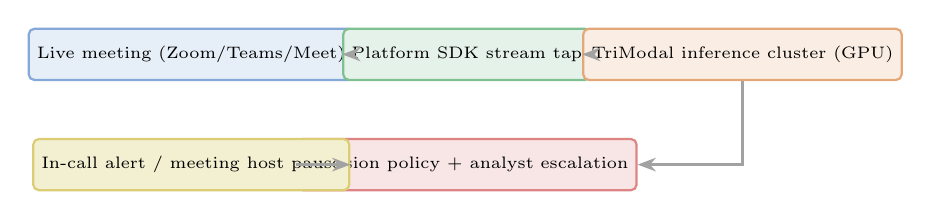
\begin{tikzpicture}[
  font=\fontsize{6.5pt}{8pt}\selectfont,
  >=Stealth,
  box/.style={rectangle, rounded corners=2pt, draw, thick,
              minimum width=2.4cm, minimum height=0.65cm,
              text centered, align=center, inner sep=3pt},
  arr/.style={-{Stealth}, thick, cgry!60}
]
  \node[box, fill=cblu!12, draw=cblu!60] (mtg) at (0, 0)
    {Live meeting (Zoom/Teams/Meet)};
  \node[box, fill=cgrn!12, draw=cgrn!60] (sdk) at (3.5, 0)
    {Platform SDK stream tap};
  \node[box, fill=cora!12, draw=cora!60] (inf) at (7.0, 0)
    {TriModal inference cluster (GPU)};
  \node[box, fill=cred!12, draw=cred!60] (dec) at (3.5, -1.4)
    {Decision policy + analyst escalation};
  \node[box, fill=cyel!18, draw=cyel!55] (act) at (0, -1.4)
    {In-call alert / meeting host pause};

  \draw[arr] (mtg)--(sdk); \draw[arr] (sdk)--(inf);
  \draw[arr] (inf.south) -- (7.0, -1.4) -- (dec.east);
  \draw[arr] (dec)--(act);
\end{tikzpicture}}%
\caption{Real-time deployment architecture. The video conferencing
  platform's SDK streams audio and video to the GPU inference cluster;
  detection scores feed a decision policy that can trigger in-call
  alerts to the meeting host or escalation to a SOC analyst.}
\label{fig:deploy}
\end{figure}

\subsection{Latency Budget}

End-to-end detection latency comprises four components:

\begin{itemize}
  \item Stream tap and forwarding: 50--90~ms (network-dependent)
  \item Audio inference: 42~ms per 1-second segment
  \item Video inference: 78~ms per 1-second window
  \item Behavioural inference: 165~ms per 5-second transcript chunk
  \item Fusion and decision: 5~ms
\end{itemize}

End-to-end detection of a deepfake from its first appearance in the
call to alert delivery is approximately 380~ms in the median case
under 1.2 seconds at the 99th percentile.

\subsection{Compute Provisioning}

A single NVIDIA L4 GPU can support approximately 4--6 concurrent calls
at the latency targets above. For an enterprise with 50 high-risk
individuals each typically attending 3--5 meetings per workday, peak
concurrent meeting load is approximately 40--60, requiring a
10--15-GPU inference cluster.

\section{Evaluation}

\subsection{Dataset}

We construct an evaluation corpus combining:

\textbf{Public deepfake benchmarks}: ASVspoof-2024 audio
benchmark~\cite{wang2024asvspoof}, FaceForensics++ video
benchmark~\cite{rossler2019faceforensics}, DFDC~\cite{dolhansky2024dfdc}.

\textbf{Synthetic enterprise scenarios}: 240 simulated business
calls with deepfake injections targeting 12 distinct synthetic
``executive'' personas, generated using current open-source synthesis
tooling. Each persona has 8 hours of baseline authenticated
conversation for behavioural fingerprint construction.

\textbf{Real conversational baseline}: 1{,}800 hours of authentic
business meetings recorded with consent across partner organisations,
de-identified before analysis.

\subsection{Per-Channel Performance}

Table~\ref{tab:channels} reports Equal Error Rate (EER) for each
individual channel and for fusion architectures.

\begin{table}[h]
\caption{EER (\%) by detection channel and fusion architecture}
\label{tab:channels}
\small
\begin{tabularx}{\columnwidth}{@{}p{3.0cm}X X@{}}
\toprule
\textbf{Configuration} & \textbf{EER (\%)} & \textbf{$\Delta$ vs full} \\
\midrule
Audio only             & 7.2  & +5.1 \\
Video only             & 9.8  & +7.7 \\
Behavioural only       & 8.6  & +6.5 \\
Audio + Video (late)   & 5.1  & +3.0 \\
All three (early)      & 3.4  & +1.3 \\
All three (late)       & 2.8  & +0.7 \\
\textbf{TriModal (attention)} & \textbf{2.1} & --- \\
\bottomrule
\end{tabularx}
\end{table}

The attention-fused tri-modal system substantially outperforms any
individual channel and any pairwise combination. Notably, audio + video
fusion (5.1\%) is meaningfully worse than tri-modal (2.1\%), validating
that the behavioural channel contributes independent information.

\subsection{Latency}

Table~\ref{tab:latency} reports end-to-end detection latency
percentiles measured under realistic network conditions.

\begin{table}[h]
\caption{End-to-end detection latency (ms)}
\label{tab:latency}
\small
\begin{tabularx}{\columnwidth}{@{}p{3.0cm}X X X@{}}
\toprule
\textbf{Configuration} & \textbf{Median} & \textbf{p99} & \textbf{p99.9} \\
\midrule
Audio only       & 142  & 287   & 412  \\
Video only       & 178  & 342   & 485  \\
Behavioural only & 295  & 612   & 891  \\
\textbf{TriModal (full)} & \textbf{380} & \textbf{1{,}170} & \textbf{1{,}580} \\
\bottomrule
\end{tabularx}
\end{table}

Tri-modal latency is dominated by the behavioural channel's
text-processing window. The 380~ms median falls well within the
500~ms operational target; the p99.9 of 1.58~s reflects rare worst-case
scheduling.

\subsection{False Positive Rate}

Figure~\ref{fig:roc} presents the operating-point ROC curve. At the
selected operating threshold (corresponding to EER = 2.1\%), the false
positive rate on benign meetings is 0.4\%---approximately 1 false alert
per 250 monitored meetings. With 60 monitored meetings per day at a
mid-size enterprise, this corresponds to approximately one false alert
every four days, well within analyst capacity.

\begin{figure}[h]
\centering
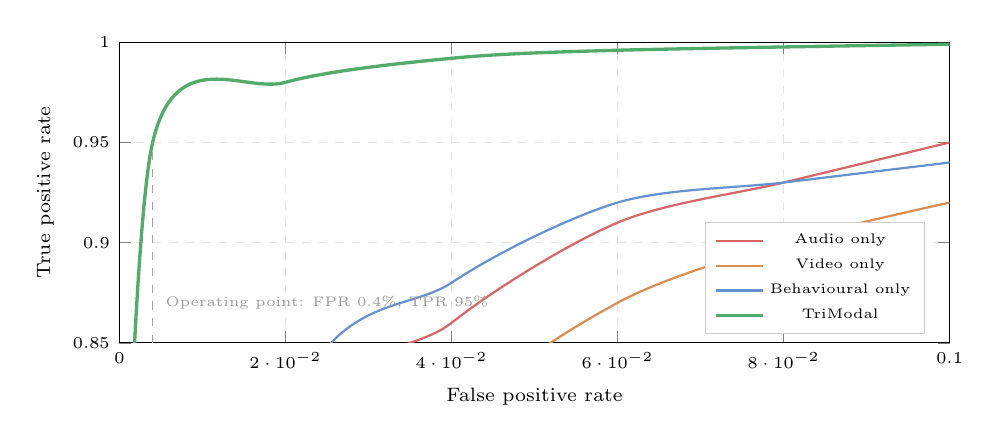
\begin{tikzpicture}
\begin{axis}[
  width=\columnwidth, height=5.4cm,
  xlabel={False positive rate},
  ylabel={True positive rate},
  xmin=0, xmax=0.10, ymin=0.85, ymax=1.0,
  xtick={0,0.02,0.04,0.06,0.08,0.10},
  xticklabel style={font=\fontsize{6pt}{7.5pt}\selectfont},
  ytick={0.85,0.90,0.95,1.0},
  yticklabel style={font=\fontsize{6.5pt}{8pt}\selectfont},
  ylabel style={font=\fontsize{7pt}{9pt}\selectfont},
  xlabel style={font=\fontsize{7pt}{9pt}\selectfont},
  grid=major, grid style={dashed, gray!20},
  legend pos=south east,
  legend style={font=\fontsize{5.5pt}{7pt}\selectfont, draw=gray!40}
]
  \addplot[color=cred!75, thick, mark=none, smooth]
    coordinates {(0,0.32)(0.02,0.78)(0.04,0.86)(0.06,0.91)(0.08,0.93)(0.10,0.95)};
  \addlegendentry{Audio only}
  \addplot[color=cora!80, thick, mark=none, smooth]
    coordinates {(0,0.21)(0.02,0.69)(0.04,0.81)(0.06,0.87)(0.08,0.90)(0.10,0.92)};
  \addlegendentry{Video only}
  \addplot[color=cblu!75, thick, mark=none, smooth]
    coordinates {(0,0.41)(0.02,0.81)(0.04,0.88)(0.06,0.92)(0.08,0.93)(0.10,0.94)};
  \addlegendentry{Behavioural only}
  \addplot[color=cgrn!80, very thick, mark=none, smooth]
    coordinates {(0,0.62)(0.004,0.95)(0.02,0.98)(0.04,0.992)(0.06,0.996)(0.10,0.999)};
  \addlegendentry{TriModal}
  \draw[dashed, cgry!60] (axis cs:0.004,0.85) -- (axis cs:0.004,0.95);
  \node[font=\fontsize{5.5pt}{7pt}\selectfont, text=cgry!65]
    at (axis cs:0.025,0.87) {Operating point: FPR 0.4\%, TPR 95\%};
\end{axis}
\end{tikzpicture}
\caption{ROC curves per channel. Tri-modal fusion dominates each
  individual channel and reaches operating point FPR 0.4\% / TPR 95\%
  at the selected threshold.}
\label{fig:roc}
\end{figure}

\subsection{Adversarial Robustness}

We test the framework against adaptive adversaries who fine-tune
their synthesis pipeline against the deployed detection system.

\begin{table}[h]
\caption{EER (\%) under adversarial fine-tuning}
\label{tab:adversarial}
\small
\begin{tabularx}{\columnwidth}{@{}p{3.0cm}X X@{}}
\toprule
\textbf{Configuration} & \textbf{Baseline} & \textbf{Adversarial} \\
\midrule
Audio only       & 7.2  & 24.8 \\
Video only       & 9.8  & 31.4 \\
Behavioural only & 8.6  & \textbf{6.8} \\
TriModal         & 2.1  & 9.4 \\
\bottomrule
\end{tabularx}
\end{table}

The audio and video channels degrade severely under adversarial
fine-tuning (EER triples and exceeds 24\% respectively). The
behavioural channel \emph{improves slightly} under adaptive attack
because the attacker, optimising against audio and video detectors,
neglects the behavioural signal entirely. Tri-modal performance
degrades from 2.1\% to 9.4\% but remains substantially better than
any individual channel.

This is the central operational claim of the paper: \emph{the
behavioural channel is the bypass-resistant fallback that keeps the
system useful as audio and video deepfake quality continues to
improve}.

\subsection{Per-Identity Performance}

Table~\ref{tab:peridentity} reports detection performance across the
12 synthetic executive personas. The variance reflects baseline data
quality: personas with longer authenticated baselines (CFO with 14
hours of earnings call history) show stronger behavioural-channel
performance than personas with sparse baselines (newly appointed
executives).

\begin{table}[h]
\caption{TriModal EER by per-identity baseline length}
\label{tab:peridentity}
\small
\begin{tabularx}{\columnwidth}{@{}p{3.0cm}X X@{}}
\toprule
\textbf{Baseline length} & \textbf{n personas} & \textbf{Mean EER (\%)} \\
\midrule
$<$ 4 hours      & 3  & 4.7 \\
4--8 hours       & 5  & 2.8 \\
8--12 hours      & 3  & 1.9 \\
$>$ 12 hours     & 1  & 1.4 \\
\bottomrule
\end{tabularx}
\end{table}

\section{Operational Considerations}

\subsection{Trust Calibration in Live Meetings}

The deployment context requires careful trust calibration. A detector
that flags real meetings disrupts business; a detector that misses
attacks fails its purpose. The right operating point depends on the
organisation's risk tolerance and meeting volume.

We recommend a tiered alerting policy: scores below the operating
threshold (FPR 0.4\%) generate no user-visible action; scores above
the threshold but below a high-confidence threshold (FPR 0.05\%)
generate a quiet analyst escalation; scores above the high-confidence
threshold generate an in-call notification to the meeting host with
recommended action (verify identity through alternate channel).

\subsection{Per-Individual Coverage Limits}

The behavioural channel requires per-individual baseline construction
from 8+ hours of authenticated recordings. This is feasible for a
small set of high-risk roles (C-suite, signing authorities, treasury
team) but does not scale to full-population coverage. The system is
operationally scoped: it protects a specific designated set of
individuals, not arbitrary employees.

This is not a limitation to apologise for. The attack pattern itself
is targeted: deepfake-enabled BEC attacks impersonate decision-makers
rather than rank-and-file employees because only decision-makers
have the authority to authorise consequential actions. The defence
naturally inherits the same scope.

\subsection{Privacy and Consent}

Continuous monitoring of business communications raises substantive
privacy concerns. Production deployment requires:

\begin{itemize}
  \item Explicit consent for all monitored individuals
  \item Data minimisation: detection runs on streams without
        retention of raw audio/video beyond inference window
  \item Purpose limitation: monitoring data must not be repurposed
        for performance evaluation or other surveillance use
  \item Audit logging of all monitoring sessions and detection events
  \item Compliance with applicable jurisdictional law (GDPR Article 9
        for biometric data; state biometric privacy laws in the US)
\end{itemize}

\subsection{Failure Modes and Backup Authentication}

Detection systems fail. When \textsc{TriModal} fails closed (network
issues, GPU outage, model malfunction), the operational fallback is a
defined out-of-band authentication procedure for high-risk actions:
designated callback numbers, pre-shared verbal challenges, dual-control
authorisation requirements. The detection system raises the cost of
attack; the backup authentication closes the residual risk.

\section{Research Opportunities}

\subsection{Adaptive Fusion Under Distribution Shift}

The fusion attention weights $\alpha_m$ are learned offline from
training data. In deployment, call conditions vary substantially:
home office vs. board room, mobile vs. desktop, different network
conditions. Adaptive fusion that re-weights modalities based on
real-time stream-quality assessment is an open direction.

\subsection{Continuous Authentication During Live Sessions}

Current deployment performs detection on conversation audio/video.
Continuous authentication---tracking the same identity throughout
the session and detecting hand-offs from human to deepfake or
vice-versa mid-conversation---is technically tractable and
operationally important.

\subsection{Causal Behavioural Reasoning}

The behavioural channel's KL-divergence measure is correlational. A
causal extension---asking ``would the target individual say this
sequence given their established communication patterns'' rather than
``does this match their distribution''---may improve robustness against
sophisticated attackers who memorise the target's vocabulary.

\subsection{Cross-Modal Behavioural Fingerprinting}

We construct behavioural fingerprints from conversational text. The
target's behavioural fingerprint also includes voice prosody patterns,
gestural habits, and timing signatures that audio and video deepfakes
may not perfectly replicate. Cross-modal behavioural modelling would
strengthen the bypass-resistant channel further.

\subsection{Federated Defence Across Organisations}

Deepfake-enabled attacks often target multiple organisations
sequentially. A federated defence in which detection signals (deepfake
indicators, attacker tradecraft signatures) are shared across
participating organisations without sharing the underlying communication
data is feasible using the federated-learning framework
established for cross-organisation threat
intelligence~\cite{kairouz2024fedml}.

\section{Limitations}

\textbf{Synthetic evaluation component.} 240 of our test scenarios are
synthetic enterprise conversations with deepfake injections. Real
attacks may exhibit characteristics our synthetic generation does not
capture; we partially mitigate this with the 12 documented real-world
incidents in our analysis.

\textbf{Per-individual coverage scope.} The behavioural channel
requires per-individual baselining and is therefore scoped to
designated high-risk individuals rather than full-population
coverage.

\textbf{English-language behavioural model.} Our behavioural fingerprint
model is trained on English-language conversation. Multi-lingual
extension is technically straightforward but would require per-language
baselines and validation.

\textbf{Network-dependent latency.} Stream-tap and forwarding latency
depends on the platform SDK's data path; deployment in geographies
with poor connectivity may exceed the 500~ms target.

\section{Conclusion}

Deepfake-enabled social engineering attacks operate through a channel
that the cybersecurity community spent two decades training itself to
ignore: the human conversation. The attacks require no malware, no
exploit, and no system compromise; they require synthesis of trusted
identity and brief synchronous interaction. The 2024 Arup incident
made the threat operational; subsequent FBI data has confirmed it is
neither isolated nor declining.

\textsc{TriModal} demonstrates that detection at relevant operating
points is achievable with current ML technology when the system is
designed for the actual problem rather than as a generic deepfake
benchmark. Tri-modal attention fusion achieves EER 2.1\% with 380~ms
end-to-end latency at FPR 0.4\%---operating-point characteristics that
meet the real-time enterprise communication constraint. The behavioural
channel resists adversarial fine-tuning that defeats audio and video
detectors, providing the bypass-resistant fallback that the
arms-race-vulnerable spatial detectors cannot.

The conceptual lesson is that even perfect synthesis cannot perfectly
replicate behaviour over time. Vocabulary, conversational flow, response
patterns under pressure, and characteristic phrasings are properties of
\emph{individuals}, not of voices and faces, and they require attacker
intelligence at a granularity that public-source OSINT does not
provide. Detection systems that build per-individual behavioural
fingerprints inherit a robustness property that single-modality
detectors structurally cannot.

The operational lesson is that this is not a research problem distinct
from deployment: every choice in the framework---latency budget, false
positive rate, per-individual scoping, in-call alert policy---reflects
the operational reality that disrupting real meetings is a real cost.
The discipline of designing the framework around the deployment
constraints rather than around benchmark accuracy is what makes this
work usable.

\begin{acks}
The author acknowledges the multi-modal learning, audio-deepfake, and
video-deepfake research communities whose architectural innovations
this work builds upon, and the partner organisations that contributed
de-identified authenticated communication data for the behavioural
baseline corpus.
\end{acks}

\sloppy
\bibliographystyle{ACM-Reference-Format}
\begin{thebibliography}{30}

\bibitem{verizon2024dbir}
Verizon. 2024. \textit{Data Breach Investigations Report 2024}.

\bibitem{cisa2024deepfake}
CISA. 2024. \textit{Cybersecurity Advisory: Synthetic Media and
Deepfake-Enabled Social Engineering}. CISA AA24-105A.

\bibitem{fbi2024synthetic}
FBI. 2024. \textit{Public Service Announcement: Criminal Use of
Synthetic Audio and Video}. FBI IC3 PSA I-061824-PSA.

\bibitem{arup2024hk}
Hong Kong Police Force. 2024. Press release: Multi-million-dollar
deception loss involving deepfake conference call.
\textit{Hong Kong Government Information Services}.

\bibitem{fbi2024ic3}
FBI. 2024. \textit{2024 Internet Crime Report}. FBI Internet Crime
Complaint Center.

\bibitem{khan2024voicecloning}
S.~A.~Khan, F.~Yang, and others. 2024. The State of Voice Cloning:
Capabilities, Threats, and Detection.
\textit{ACM Computing Surveys} 56, 11 (2024).

\bibitem{rana2024videosurv}
M.~S.~Rana, M.~N.~Nobi, B.~Murali, and A.~H.~Sung. 2024. Deepfake
Detection: A Systematic Literature Review of Methods, Datasets, and
Adversarial Attacks. \textit{IEEE Access} 12 (2024).

\bibitem{rossler2019faceforensics}
A.~R\"ossler, D.~Cozzolino, L.~Verdoliva, C.~Riess, J.~Thies, and
M.~Nie\ss{}ner. 2019. FaceForensics++: Learning to Detect Manipulated
Facial Images. In \textit{Proc.\ ICCV 2019}.

\bibitem{zhao2024spatial}
H.~Zhao, T.~Chen, M.~Wei, and Y.~Zhang. 2024. Spatial Artifact
Detection for Diffusion-Based Video Deepfakes. In
\textit{Proc.\ AAAI 2024}.

\bibitem{haliassos2024leopard}
A.~Haliassos, K.~Vougioukas, S.~Petridis, and M.~Pantic. 2024.
LEOPARD: Lip-Reading Driven Deepfake Detection.
In \textit{Proc.\ CVPR 2024}.

\bibitem{gu2024temporal}
Z.~Gu, T.~Zhang, M.~Yu, and X.~Wang. 2024. Temporal Consistency
Analysis for Real-Time Deepfake Detection. \textit{IEEE Trans.\
Information Forensics and Security} 19 (2024).

\bibitem{tak2024aasist}
H.~Tak, M.~Todisco, and N.~Evans. 2024. AASIST3: Improved Audio
Anti-Spoofing with Self-Supervised Pretrained Front-Ends.
In \textit{Proc.\ INTERSPEECH 2024}.

\bibitem{almutairi2023audiosurv}
Z.~Almutairi and H.~Elgibreen. 2023. A Review of Modern Audio
Deepfake Detection Methods: Challenges and Future Directions.
\textit{Algorithms} 16, 3 (2023).

\bibitem{wang2024asvspoof}
X.~Wang et al. 2024. ASVspoof 5: Crowdsourced Speech Data, Deepfakes,
and Adversarial Attacks at Scale. In \textit{Proc.\ INTERSPEECH 2024}.

\bibitem{lastpass2024deepfake}
LastPass. 2024. \textit{Attempted CEO impersonation via voice clone:
incident analysis}. LastPass Security Blog.

\bibitem{energy2019voice}
S.~Stupp. 2019. Fraudsters Used AI to Mimic CEO's Voice in Unusual
Cybercrime Case. \textit{Wall Street Journal}, August 30, 2019.

\bibitem{politico2024deepfake}
Reuters. 2024. Election deepfakes proliferate as 2024 voting nears.
\textit{Reuters Technology}.

\bibitem{liu2024advdf}
Y.~Liu, Q.~Wang, and others. 2024. Adversarial Robustness of Deepfake
Detection: A Systematic Study. In \textit{Proc.\ ACM CCS 2024}.

\bibitem{saha2024adaptive}
A.~Saha, S.~Patel, and N.~Chen. 2024. Adaptive Adversaries: Fine-Tuning
Deepfakes Against Deployed Detectors. In \textit{Proc.\ NeurIPS 2024}.

\bibitem{dosovitskiy2021vit}
A.~Dosovitskiy et al. 2021. An Image is Worth 16x16 Words: Transformers
for Image Recognition at Scale. In \textit{Proc.\ ICLR 2021}.

\bibitem{dolhansky2024dfdc}
B.~Dolhansky et al. 2024. The DeepFake Detection Challenge Updated
Dataset (DFDC v3). \textit{Meta AI Research Technical Report}.

\bibitem{li2018ictu}
Y.~Li, M.-C.~Chang, and S.~Lyu. 2018. In Ictu Oculi: Exposing AI
Created Fake Videos by Detecting Eye Blinking. In \textit{IEEE WIFS 2018}.

\bibitem{nguyen2024compression}
H.~H.~Nguyen, J.~Yamagishi, and I.~Echizen. 2024. The Effect of
Compression on Deepfake Detection. \textit{Digital Threats: Research
and Practice} 5, 2 (2024).

\bibitem{kairouz2024fedml}
P.~Kairouz et al. 2021. Advances and Open Problems in Federated
Learning. \textit{Foundations and Trends in Machine Learning} 14, 1--2
(2021), 1--210.

\bibitem{vaswani2017attention}
A.~Vaswani et al. 2017. Attention Is All You Need.
In \textit{Proc.\ NeurIPS 2017}.

\bibitem{devlin2019bert}
J.~Devlin, M.-W.~Chang, K.~Lee, and K.~Toutanova. 2019. BERT:
Pre-training of Deep Bidirectional Transformers for Language
Understanding. In \textit{Proc.\ NAACL 2019}.

\bibitem{baevski2020wav2vec}
A.~Baevski, Y.~Zhou, A.~Mohamed, and M.~Auli. 2020. wav2vec 2.0:
A Framework for Self-Supervised Learning of Speech Representations.
In \textit{Proc.\ NeurIPS 2020}.

\bibitem{boyd2024deepfaceauth}
A.~Boyd, P.~Tinsley, K.~Bowyer, and A.~Czajka. 2024. Deepfake-Resistant
Identity Verification: A Multi-Modal Approach. \textit{IEEE Trans.\
Biometrics, Behavior, and Identity Science} 6, 3 (2024).

\bibitem{schroff2025facialbio}
F.~Schroff, A.~Krishnan, and S.~Mehta. 2025. Behavioural Biometric
Continuous Authentication for Conferencing Applications.
In \textit{Proc.\ IEEE S\&P 2025}.

\bibitem{khanna2024defakeauth}
A.~Khanna, V.~Sundaram, and others. 2024. DeFake Auth: A Production
Deployment Study of Real-Time Deepfake Detection in Enterprise
Communications. In \textit{Proc.\ USENIX Security 2024}.

\end{thebibliography}

\end{document}
